%  LaTeX support: latex@mdpi.com 
%  In case you need support, please attach all files 
%  that are necessary for compiling as well as the log file, 
%  and specify the details of your LaTeX setup 
%  (which operating system and LaTeX version / tools you are using).

%=================================================================
\documentclass[ijgi,article,submit,moreauthors,pdftex]{Definitions/mdpi} 


%=================================================================
\firstpage{1} 
\makeatletter 
\setcounter{page}{\@firstpage} 
\makeatother
\pubvolume{xx}
\issuenum{1}
\articlenumber{5}
\pubyear{2019}
\copyrightyear{2019}
%\externaleditor{Academic Editor: name}
\history{Received: date; Accepted: date; Published: date}
%\updates{yes} % If there is an update available, un-comment this line

%% MDPI internal command: uncomment if new journal that already uses continuous page numbers 
%\continuouspages{yes}

%------------------------------------------------------------------
% The following line should be uncommented if the LaTeX file is uploaded to arXiv.org
%\pdfoutput=1

%=================================================================
% Add packages and commands here. The following packages are loaded in our class file: fontenc, calc, indentfirst, fancyhdr, graphicx, lastpage, ifthen, lineno, float, amsmath, setspace, enumitem, mathpazo, booktabs, titlesec, etoolbox, amsthm, hyphenat, natbib, hyperref, footmisc, geometry, caption, url, mdframed, tabto, soul, multirow, microtype, tikz

\usepackage{xspace}


%=================================================================
%% Please use the following mathematics environments: Theorem, Lemma, Corollary, Proposition, Characterization, Property, Problem, Example, ExamplesandDefinitions, Hypothesis, Remark, Definition, Notation, Assumption
%% For proofs, please use the proof environment (the amsthm package is loaded by the MDPI class).




\graphicspath{{images/}}

\newcommand{\Astar}{A$^{\!\star}$\xspace}

\newcommand{\e}[1]{\times 10^{#1}}
\newcommand{\fig}{Figure~}
\newcommand{\eq}{Equation~}
\newcommand{\fo}{Formula~}
\newcommand{\sect}{Section~}
\newcommand{\mytable}{Table~}
\newcommand{\chap}{Chapter~}
\newcommand{\figs}{Figures~}
\newcommand{\eqs}{Equations~}
\newcommand{\fos}{Formulas~}
\newcommand{\sects}{Sections~}
\newcommand{\tabs}{Tables~}
\newcommand{\chaps}{Chapters~}


%=================================================================
% Full title of the paper (Capitalized)
\Title{Finding parallel events of merging land-cover parcels 
to support smooth zooming}

% Author Orchid ID: enter ID or remove command
\newcommand{\orcidauthorA}{0000-0000-000-000X} % Add \orcidA{} behind the author's name
%\newcommand{\orcidauthorB}{0000-0000-000-000X} % Add \orcidB{} behind the author's name

% Authors, for the paper (add full first names)
\Author{
Firstname Lastname $^{1,\dagger,\ddagger}$\orcidA{}, 
Firstname Lastname $^{1,\ddagger}$ and 
Firstname Lastname $^{2,}$*}

% Authors, for metadata in PDF
\AuthorNames{Firstname Lastname, Firstname Lastname and Firstname Lastname}

% Affiliations / Addresses (Add [1] after \address if there is only one affiliation.)
\address{%
$^{1}$ \quad Affiliation 1; e-mail@e-mail.com\\
$^{2}$ \quad Affiliation 2; e-mail@e-mail.com}

% Contact information of the corresponding author
\corres{Correspondence: e-mail@e-mail.com; Tel.: (optional; include country code; 
if there are multiple corresponding authors, add author initials) +xx-xxxx-xxx-xxxx (F.L.)}

% Current address and/or shared authorship
\firstnote{Current address: Affiliation 3} 
\secondnote{These authors contributed equally to this work.}
% The commands \thirdnote{} till \eighthnote{} are available for further notes

%\simplesumm{} % Simple summary

%\conference{} % An extended version of a conference paper

% Abstract (Do not insert blank lines, i.e. \\) 
\abstract{
%meaning of time.
Land-cover parcels are important features on maps.
When users zoom out on digital maps, 
some land-cover parcels become too tiny to be seen, 
which result in visual clutters. 
To avoid this problem, 
we merge small parcels into their neighbors to form larger parcels. 
We define an \emph{event} as merging a small parcel into a neighbor, 
where the color of the small parcel gradually changes 
to the color of the neighbor
or the neighbor gradually expands over the small parcel.
However, because of the given sequence 
in which the events are processed one by one, 
the map users still experience shock changes 
(because the merging transition time of their zooming out can be short).
We try to produce smooth changes by paralleling the events.
We define a \emph{step} as a set of merging events happening at the same time.
In our method, a merging step is completely processed 
before the next merging step takes place (all sequential). 
In this way, each event has more time to be observed by users,
resulting in more smooth zooming. 
Furthermore, we require that 
all the pairs of parcels involved in the merging events of a step 
do not have any common neighbors, 
which makes the merging events independent from each other.
There are two benefits of this independency.
First, it is easy for us to maintain the topology of the map.
Second, users can more easily understand the events 
than merging several parcels into a single one.
This paper shows the details of finding and processing parallel events.
Then, this paper compares between the scale transitions of maps generated
based on single-event merging step and parallel-event merging step.
Our original contribution is the proposal of the parallel generalization
maintaining map consistency over scale change. 
%why? how? what? so what?
}

% Keywords
\keyword{Map generalization, Vario-scale maps, Continuous generalization}



%%%%%%%%%%%%%%%%%%%%%%%%%%%%%%%%%%%%%%%%%%
% Only for the journal Data:
%\dataset{DOI number or link to the deposited data set in cases where the data set is published or set to be published separately. If the data set is submitted and will be published as a supplement to this paper in the journal Data, this field will be filled by the editors of the journal. In this case, please make sure to submit the data set as a supplement when entering your manuscript into our manuscript editorial system.}

%\datasetlicense{license under which the data set is made available (CC0, CC-BY, CC-BY-SA, CC-BY-NC, etc.)}



%\setcounter{secnumdepth}{4}
%%%%%%%%%%%%%%%%%%%%%%%%%%%%%%%%%%%%%%%%%%
\begin{document}
%%%%%%%%%%%%%%%%%%%%%%%%%%%%%%%%%%%%%%%%%%



\section{Introduction}

Land-cover parcels are importance on maps. 
When users zoom out,
some land-cover parcels become too tiny to be seen,
which result in visual clutter.
We try to avoid it
by merging parcels one by one during zooming out
(see \fig\ref{fig:aggregation_sequence}).
Also, this gradual fashion allows users 
to follow the zooming more easily.
Data structure Space Scale Cube \citep{vanOosterom2014tGAPSSC} 
can be used to store the merging sequence and 
to output a map at any scale.

\begin{figure}[htb]
\centering
\includegraphics[page=2]{Intro}
\caption{An merging sequence of land-cover parcels; 
taken from \citet[][\sect1.3]{Peng2019Thesis}.}
\label{fig:aggregation_sequence}
\end{figure}

When users zoom on maps, 
they do not want to wait for too long 
in order to see the next level.
For example, they may not want to wait for more than one second,
but there may be 50 merging steps happening in the time interval
(400 steps in total for all the time intervals).
For a user, it feels like a shock change 
if all the 50 steps happen on the screen in the one second.
A nice way to solve this problem is to parallel the merging steps
(see \fig\ref{fig:parallel_comparison});
if we can select 50 steps (of the 400 steps) 
fairly evenly distributed on the whole map, 
then there may be only two steps happening on the screen,
which is easy for users to understand the change.
In this way, we repeat finding parallel merging steps 
for all the 400 steps.
A simple way to find parallel steps is to employ a greedy algorithm.
If we want to find parallel steps of higher quality, 
then we need to use some optimization.

\begin{figure}[htb]
\centering
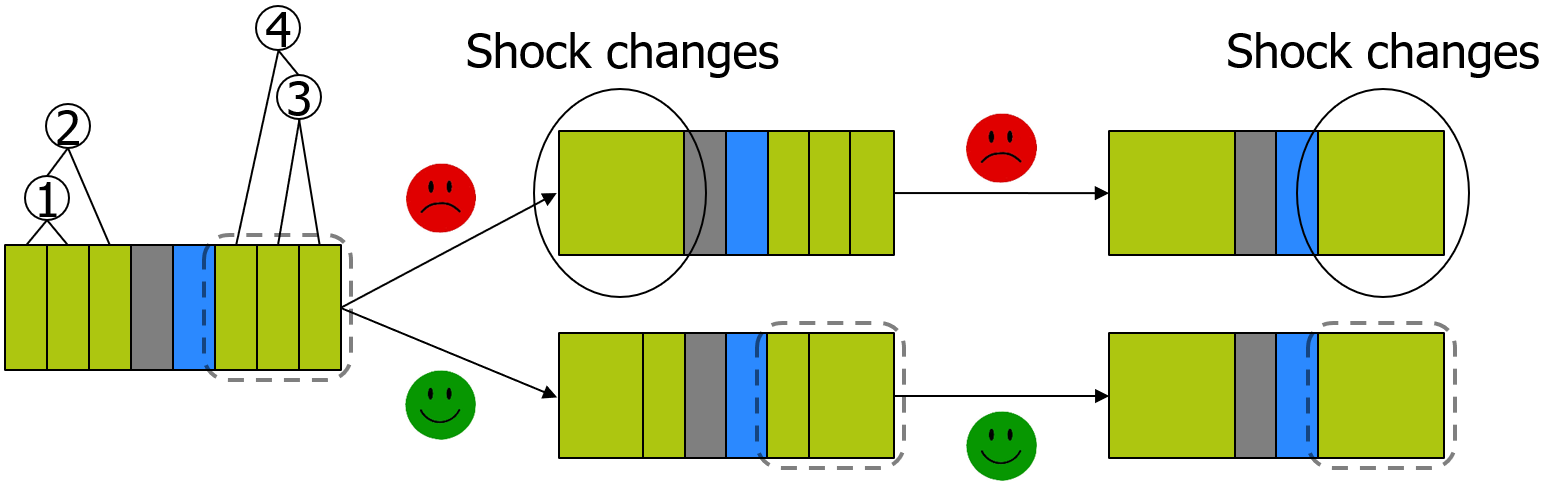
\includegraphics[width=\columnwidth]{parallel_comparison}
\caption{Processing merging steps in a sequential way (above) or a parallel way (below). 
The numbers indicate the merging sequence.
We suppose that a user is focusing on the region marked by the dashed gray polygon.}
\label{fig:parallel_comparison}
\end{figure}

We define that an merging event consists of 
one or more merging steps happening at the same time.
Some research questions are as follows.
What aspects should we optimize 
(e.g., minimizing the number of merging events or 
assigning similar numbers of merging steps to each event)?
What algorithm should we use 
(e.g., dynamic programming, \Astar, or integer linear programming)?
How much time is gained for users to observe the merging steps on the screen?
How to store the parallel merging steps?
 
\section{Related Work}
\citet{vanOosterom2005} proposed a greedy algorithm 
to merge land-cover parcels one by one.
In each iteration, that algorithm takes the least important parcel and 
merges it into the most compatible neighbor.
The importance of a parcel is defined 
based on both the area and the type of the parcel.
The compatibility between a pair of parcels is defined based on 
both the length of the common boundary and the similarity of the types 
of the pair of parcels. 
\citet[\chap2]{Peng2019Thesis} tried to find an optimal sequence 
to merge land-cover parcels
based on the \Astar algorithm or an integer linear program.
A comparison to a greedy algorithm showed that 
the \Astar algorithm improves the quality of the merging sequences.
\citet{vanOosterom2014Support} pointed out that sequentially merging
land-cover parcels may result in a suboptimal smooth-zoom effect.
To provide better visualization, they suggested that
the merging operations should be paralleled.
Then, one question is how many operations 
should be paralleled for a given scale.



\citet{Suba2014Merge} proposed three methods to merge two parcels, 
which are the ``Single flat plane'', the ``Zipper'', and the ``Eater''.
Basically, the \emph{winner} gradually expands over the \emph{loser}.
We will use the ``Eater'' because it works for all kinds of polygons 
while the other two methods have limitation in terms of the type of a polygon.
For example, the two other methods do not work for some concave polygons.



\citet{Suba2016Road} continuously generalized a planar map.
At each step, they process the least-important face.
Taking into account the condition of the face,
they put it back with higher importance, collapse it, 
or merge it into an adjacent face.
In addition to the generalization, 
they also observed the number of faces,
the area of faces, the number of road faces, the number of road edges,
and the number of operations (merge and split) 
when the scale of the map is decreasing.
These statistics can be good benchmarks for (continuous) map generalization.



\citet{Huang2016Webmap} described their strategy of implementing online maps, 
considering both the server side and the client side.

\citet{Huang2017Matrix} used a matrix to guide 
both pruning rivers and removing vertices for a river network, 
where the rows and the columns respectively represent
the rivers and the vertices.
According to the matrix, 
they were able to decide which rivers and vertices 
should be remained for a given scale.
To this purpose, they proposed a method 
to compute how many rivers and vertices 
should be kept according to that given scale.

\citet{Thiemann2018LandCover}


%\citet{Meijers2015Parallel}

%

\section{A Greedy Algorithm}

%We define an \emph{event} as merging a small parcel into a neighbor, 
%where the color of the small parcel gradually changes 
%to the color of the neighbor
%or the neighbor gradually expands over the small parcel.
%However, because of the given sequence 
%in which the events are processed one by one, 
%the map users still experience shock changes 
%(because the merging transition time of their zooming out can be short).
%We try to produce smooth changes by paralleling the events.
%We define a \emph{step} as a set of merging events happening at the same time.
%In our method, a merging step is completely processed 
%before the next merging step takes place (all sequential). 
%In this way, each event has more time to be observed by users,
%resulting in more smooth zooming. 
%Furthermore, we require that 
%all the pairs of parcels involved in the merging events of a step 
%do not have any common neighbors, 
%which makes the merging events independent from each other.
%There are two benefits of this independency.
%First, it is easy for us to maintain the topology of the map.
%Second, users can more easily understand the events 
%than merging several parcels into a single one.


We define an \emph{event} as merging a small parcel into a neighbor.
For example, 
We define a \emph{step} as 
a set of merging events happening at the same time.

\begin{figure}[htb]
\centering
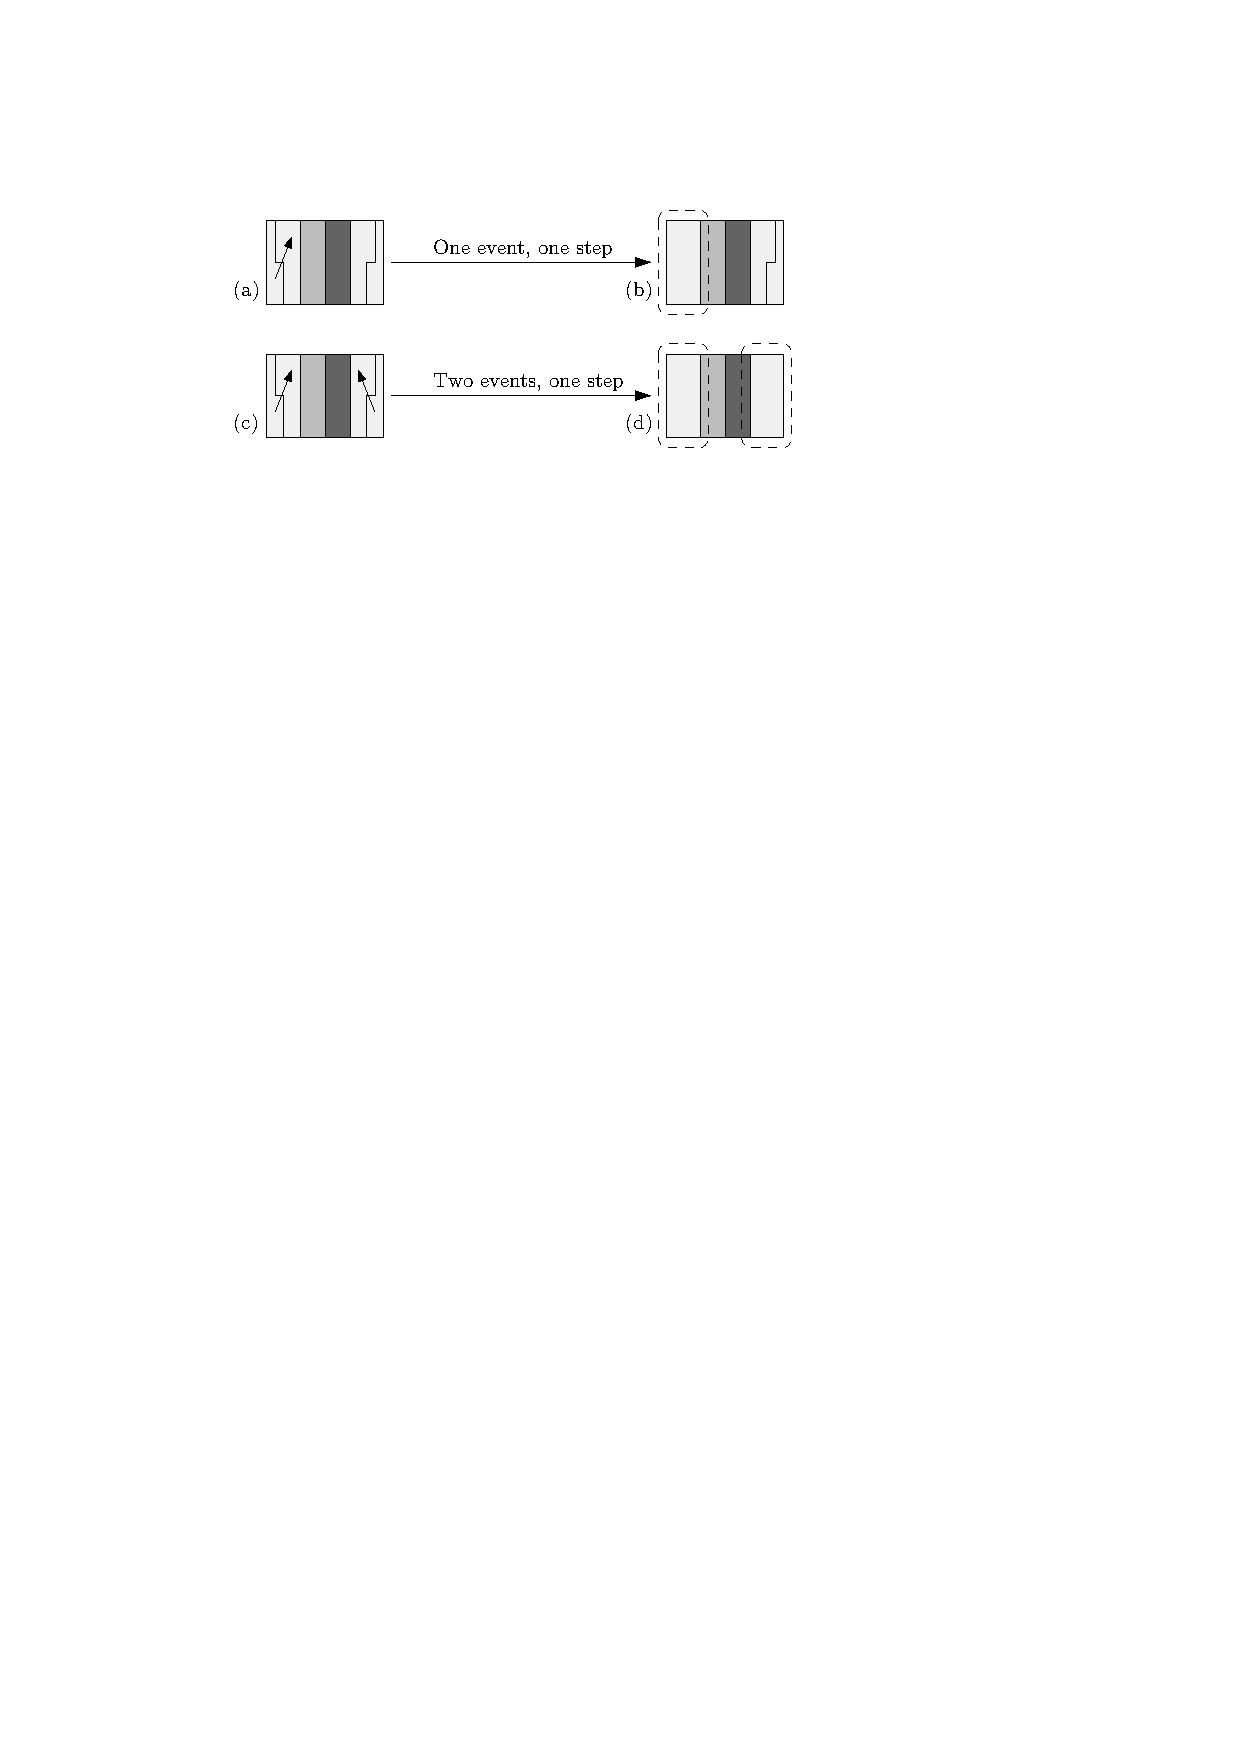
\includegraphics[page=1]{greedy_algorithm}
\caption{Merging event and merging step. 
Figure (b) is obtained }
\label{fig:greedy_algorithm}
\end{figure}

We may have $400$ merging events.
An merging step consists of one or many merging events.
We would like the steps to be as few as possible.


When a pair of polygons have been selected for an merging event, 
some polygons need to be blocked (see \fig\ref{fig:bloked_polygons}).
First, the pair of two polygons are blocked so that
they will not be selected for another merging event.
Second, the adjacent polygons of the pair of polygons are blocked.
The reason is that, when a pair of polygons have been merged, 
we must update the adjacent polygons in order to maintain the topology.
If an adjacent polygon is involved in another merging event,
then it will be a mess to update for the two merging events.
Third, the neighbors (except the initial pair of polygons) 
of the adjacent polygons are blocked.
The reason is that if a neighbor is involved in an merging event,
then an adjacent polygon will be updated from two merging events,
which may bring conflicts.

Our algorithm for an merging step works as follows.
The algorithm selects the smallest polygon and finds the most-compatible adjacent polygon.
The algorithm define an merging event based on this pair of polygons 
and blocks the surrounding polygons.
Based on the unblocked polygons, the algorithm defines another merging event.
This process is iterated 
until the (users-specified) maximum number of merging events is reached or 
there is no available merging event anymore.
Up to this point, finding merging events for an merging step is finished.
Then the blocked polygons are released, and the finding for the next steps starts.


\begin{figure}[htb]
\centering
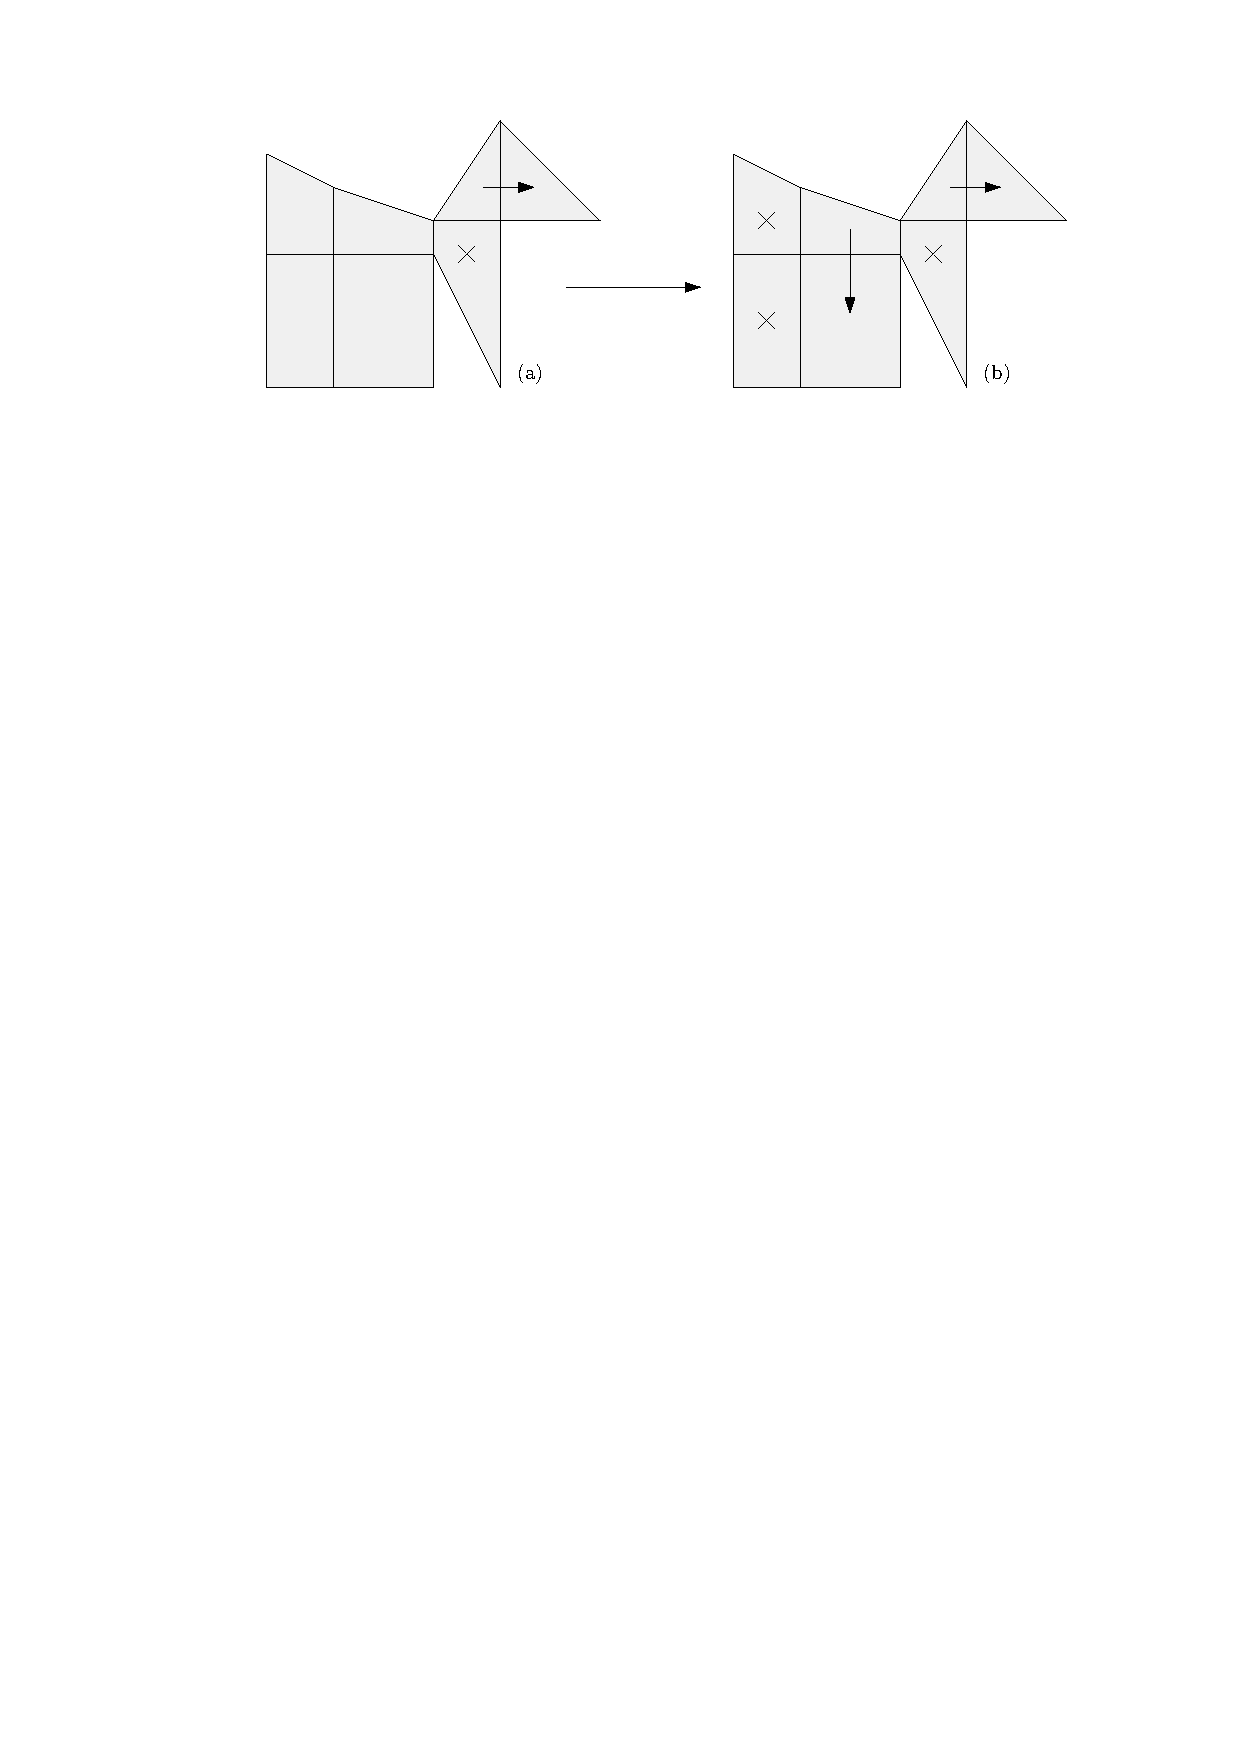
\includegraphics[]{blocked_polygons}
\caption{At a step, once the dark parcels are selected for merging, 
the neighbors are blocked for being involved for parallel events at the same step,
which makes it easy for us to maintain the topology of a map.}
\label{fig:bloked_polygons}
\end{figure}




%From the ordered sequence of the events, 
%we pick one by one if the later one will not 
%conflict with any of the previous events.
%
%We show how to find merging events for an merging step.
%We save all the adjacencies in a dictionary, say, $D_\mathrm{adj}$.
%We save all the neighbors of the involved patches of the selected events 
%in another dictionary, say, $D_\mathrm{nbr}$.
%For an event, we check if the adjacency of the two patches 
%exists in $D_\mathrm{adj}$.
%If so, and if no neighbor of the two patches exists in $D_\mathrm{nbr}$,
%then we add this event to the current merging step;
%otherwise, we skip this event for now.
%When we add this event, we also add all the neighbors of the two patches
%into dictionary $D_\mathrm{nbr}$.
%
%Two events conflict if they share a neighbor.



\section{Smooth Merging}



\begin{figure}[htb]
\centering
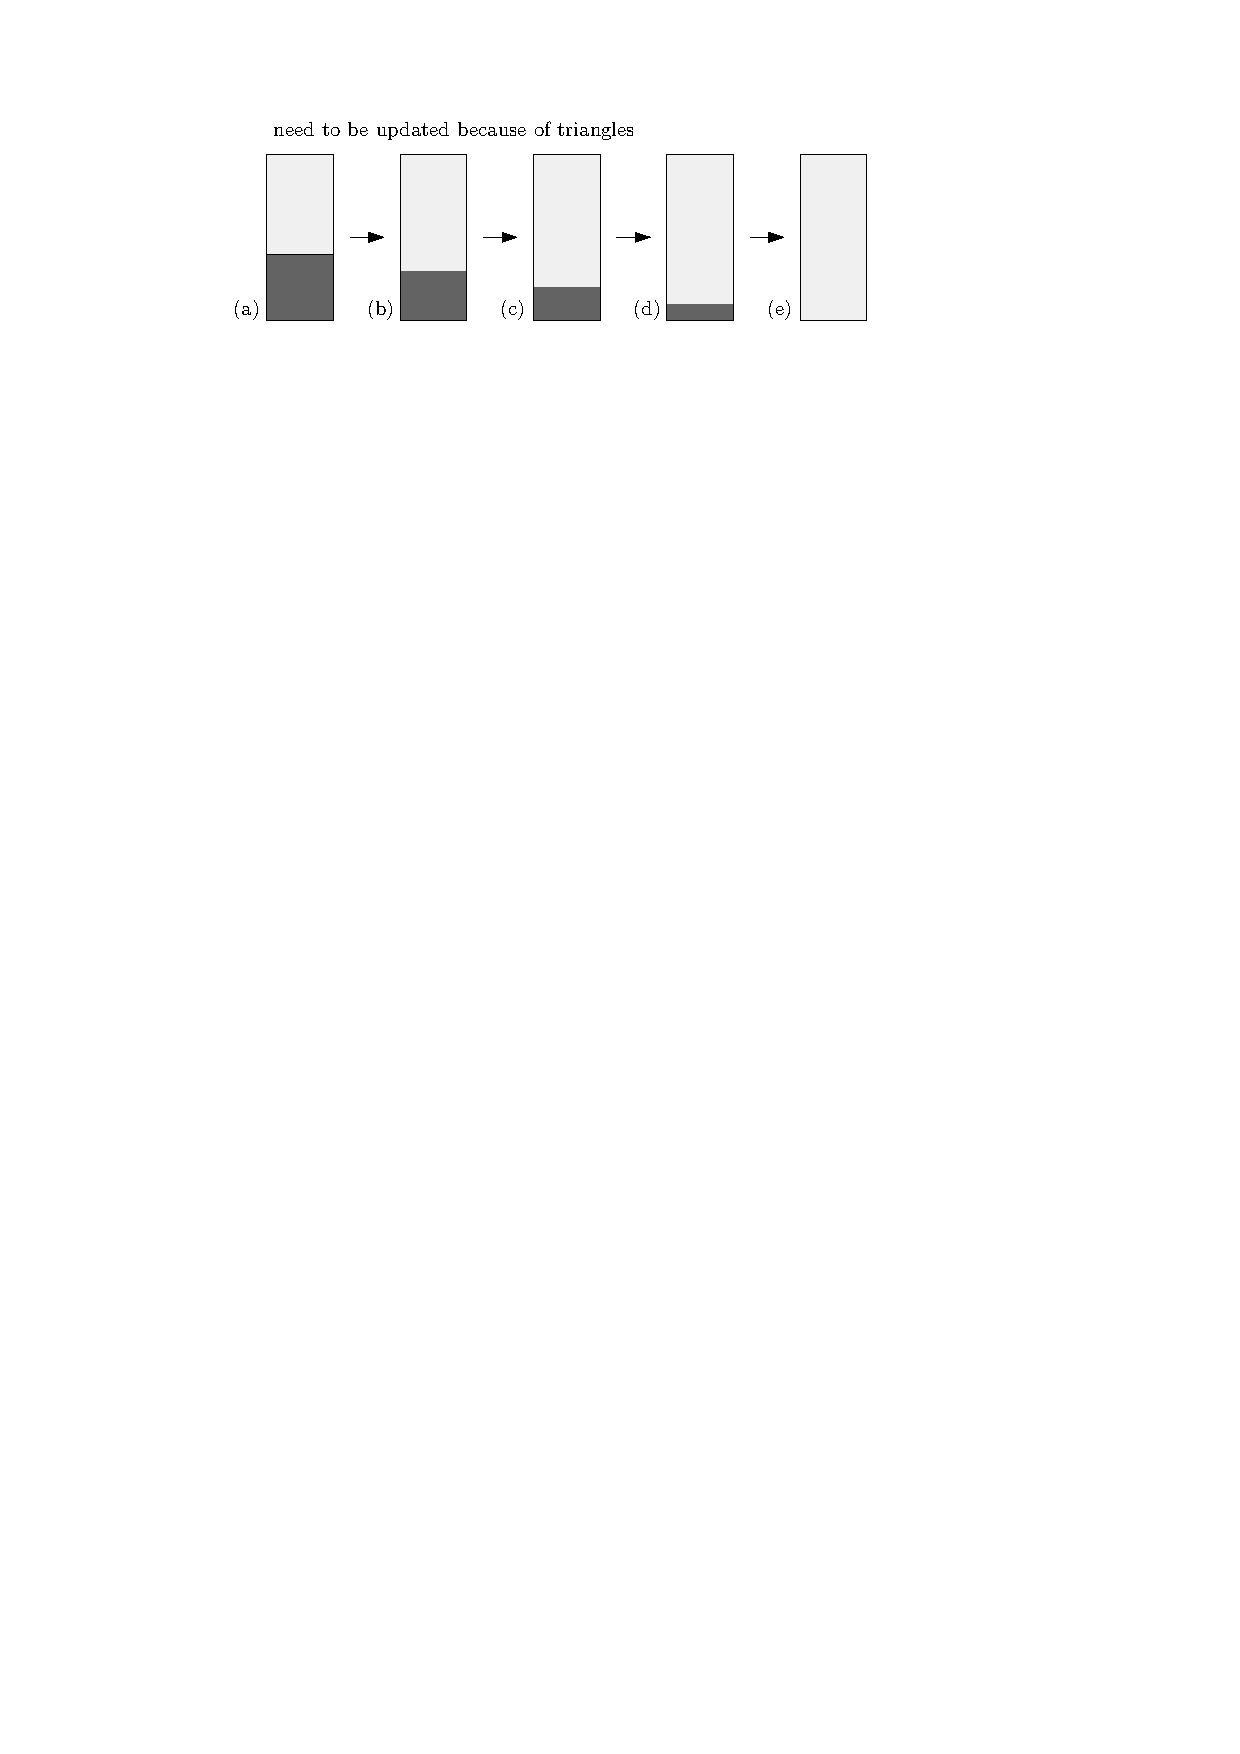
\includegraphics[page=1]{smooth_merging}
\caption{At a step, once the dark parcels are selected for merging, 
the neighbors are blocked for being involved for parallel events at the same step,
which makes it easy for us to maintain the topology of a map.}
\label{fig:smooth_merging}
\end{figure}


\section{Snapping to Certain Steps}
We may have $400$ merging events.


\section{Case Study}

The number of times that we compromised.
Because some polygons are blocked during finding merging events, 
the smallest polygon selected for an merging event 
is not the real smallest polygon 
among all the polygons at that step. 
This situation happens $XXX$ times in our data.
For the same reason, we cannot always use the most compatible adjacent polygon,
which happens $XXX$ times.

\section{Concluding Remarks}

\subsection{Future Work}

\citet{vanOosterom2005} and \citet[\chap2]{Peng2019Thesis}
respectively developed a greedy algorithm and an \Astar algorithm to find
merging sequences for land-cover parcels.
For those given merging sequence,
it is interesting to parallel some of the merging events.

Integrate split operation into our method.

evenly distribute the merging events for each step

When we remove a triangle by slicing the SSC, 
we may want to keep three vertices of the triangle instead of making four vertices.
In this case, the polyhedron (with five faces) should have curly edges,
which is also known as a \emph{curved polyhedron}.
$\cos, \sin$.



\begin{figure}[htb]
\centering
\includegraphics[page=2]{smooth_merging}
\caption{At a step, once the dark parcels are selected for merging, 
the neighbors are blocked for being involved for parallel events at the same step,
which makes it easy for us to maintain the topology of a map.}
\label{fig:smooth_merging_future}
\end{figure}

%%%%%%%%%%%%%%%%%%%%%%%%%%%%%%%%%%%%%%%%%%%
%\section{Patents}
%This section is not mandatory, but may be added if there are patents resulting from the work reported in this manuscript.
%
%%%%%%%%%%%%%%%%%%%%%%%%%%%%%%%%%%%%%%%%%%%
%\vspace{6pt} 
%
%%%%%%%%%%%%%%%%%%%%%%%%%%%%%%%%%%%%%%%%%%%
%%% optional
%%\supplementary{The following are available online at \linksupplementary{s1}, Figure S1: title, Table S1: title, Video S1: title.}
%
%% Only for the journal Methods and Protocols:
%% If you wish to submit a video article, please do so with any other supplementary material.
%% \supplementary{The following are available at \linksupplementary{s1}, Figure S1: title, Table S1: title, Video S1: title. A supporting video article is available at doi: link.}
%
%%%%%%%%%%%%%%%%%%%%%%%%%%%%%%%%%%%%%%%%%%%
%\authorcontributions{For research articles with several authors, a short paragraph specifying their individual contributions must be provided. The following statements should be used ``conceptualization, X.X. and Y.Y.; methodology, X.X.; software, X.X.; validation, X.X., Y.Y. and Z.Z.; formal analysis, X.X.; investigation, X.X.; resources, X.X.; data curation, X.X.; writing--original draft preparation, X.X.; writing--review and editing, X.X.; visualization, X.X.; supervision, X.X.; project administration, X.X.; funding acquisition, Y.Y.'', please turn to the  \href{http://img.mdpi.org/data/contributor-role-instruction.pdf}{CRediT taxonomy} for the term explanation. Authorship must be limited to those who have contributed substantially to the work reported.}
%
%%%%%%%%%%%%%%%%%%%%%%%%%%%%%%%%%%%%%%%%%%%
%\funding{Please add: ``This research received no external funding'' or ``This research was funded by NAME OF FUNDER grant number XXX.'' and  and ``The APC was funded by XXX''. Check carefully that the details given are accurate and use the standard spelling of funding agency names at \url{https://search.crossref.org/funding}, any errors may affect your future funding.}
%
%%%%%%%%%%%%%%%%%%%%%%%%%%%%%%%%%%%%%%%%%%%
%\acknowledgments{In this section you can acknowledge any support given which is not covered by the author contribution or funding sections. This may include administrative and technical support, or donations in kind (e.g., materials used for experiments).}
%
%%%%%%%%%%%%%%%%%%%%%%%%%%%%%%%%%%%%%%%%%%%
%\conflictsofinterest{Declare conflicts of interest or state ``The authors declare no conflict of interest.'' Authors must identify and declare any personal circumstances or interest that may be perceived as inappropriately influencing the representation or interpretation of reported research results. Any role of the funders in the design of the study; in the collection, analyses or interpretation of data; in the writing of the manuscript, or in the decision to publish the results must be declared in this section. If there is no role, please state ``The funders had no role in the design of the study; in the collection, analyses, or interpretation of data; in the writing of the manuscript, or in the decision to publish the results''.} 
%
%%%%%%%%%%%%%%%%%%%%%%%%%%%%%%%%%%%%%%%%%%%
%%% optional
%\abbreviations{The following abbreviations are used in this manuscript:\\
%
%\noindent 
%\begin{tabular}{@{}ll}
%MDPI & Multidisciplinary Digital Publishing Institute\\
%DOAJ & Directory of open access journals\\
%TLA & Three letter acronym\\
%LD & linear dichroism
%\end{tabular}}
%
%%%%%%%%%%%%%%%%%%%%%%%%%%%%%%%%%%%%%%%%%%%
%%% optional
%\appendixtitles{no} %Leave argument "no" if all appendix headings stay EMPTY (then no dot is printed after "Appendix A"). If the appendix sections contain a heading then change the argument to "yes".
%\appendix
%\section{}
%\unskip
%\subsection{}
%The appendix is an optional section that can contain details and data supplemental to the main text. For example, explanations of experimental details that would disrupt the flow of the main text, but nonetheless remain crucial to understanding and reproducing the research shown; figures of replicates for experiments of which representative data is shown in the main text can be added here if brief, or as Supplementary data. Mathematical proofs of results not central to the paper can be added as an appendix.
%
%\section{}
%All appendix sections must be cited in the main text. In the appendixes, Figures, Tables, etc. should be labeled starting with `A', e.g., Figure A1, Figure A2, etc. 

%%%%%%%%%%%%%%%%%%%%%%%%%%%%%%%%%%%%%%%%%%
% Citations and References in Supplementary files are permitted provided that they also appear in the reference list here. 

%=====================================
% References, variant A: internal bibliography
%=====================================
%\reftitle{References}
%\begin{thebibliography}{999}
%% Reference 1
%\bibitem[Author1(year)]{ref-journal}
%Author1, T. The title of the cited article. {\em Journal Abbreviation} {\bf 2008}, {\em 10}, 142--149.
%% Reference 2
%\bibitem[Author2(year)]{ref-book}
%Author2, L. The title of the cited contribution. In {\em The Book Title}; Editor1, F., Editor2, A., Eds.; Publishing House: City, Country, 2007; pp. 32--58.
%\end{thebibliography}
\bibliography{Reference/BibReference}

% The following MDPI journals use author-date citation: Arts, Econometrics, Economies, Genealogy, Humanities, IJFS, JRFM, Laws, Religions, Risks, Social Sciences. For those journals, please follow the formatting guidelines on http://www.mdpi.com/authors/references
% To cite two works by the same author: \citeauthor{ref-journal-1a} (\citeyear{ref-journal-1a}, \citeyear{ref-journal-1b}). This produces: Whittaker (1967, 1975)
% To cite two works by the same author with specific pages: \citeauthor{ref-journal-3a} (\citeyear{ref-journal-3a}, p. 328; \citeyear{ref-journal-3b}, p.475). This produces: Wong (1999, p. 328; 2000, p. 475)

%=====================================
% References, variant B: external bibliography
%=====================================
%\externalbibliography{yes}
%\bibliography{your_external_BibTeX_file}

%%%%%%%%%%%%%%%%%%%%%%%%%%%%%%%%%%%%%%%%%%
%% optional
%\sampleavailability{Samples of the compounds ...... are available from the authors.}

%% for journal Sci
%\reviewreports{\\
%Reviewer 1 comments and authors’ response\\
%Reviewer 2 comments and authors’ response\\
%Reviewer 3 comments and authors’ response
%}




%%%%%%%%%%%%%%%%%%%%%%%%%%%%%%%%%%%%%%%%%%
\end{document}

